	LTI filters in general are usually defined as sums of products.
	Several quantities are useful to understand their characteristics

	\subsection{Notations}
		The entire report will use several notations and conventions:
		\begin{itemize}
			\item in signal processing, t is the common notation for continue time and k the notation for discrete time. This report keeps this convention.
			\item $\langle\langle\mathcal{H}\rangle\rangle _{WCPG}$ is the worst case peak gain of the filter $\mathcal{H}$
			\item y is an output variable
			\item x is a state variable
			\item t is an intermediate variable
			\item a bold symbol (for example $\boldsymbol{h}$) denotes a matrix, that may be a vector
			\item a normal symbol (for example $\varepsilon_{t_1}(k)$) denotes a single value
		\end{itemize}

	\subsection{Reminders about signal processing}
	\begin{thdef}\label{sig} (Signal)
		Generally, a signal is a temporal variable, which takes a value from $\mathbb{R}$ at each time t.
		x(t) denotes the value of the signal x at the instant t.
		When dealing with discrete time events, the time will be represented by k.
		Then x(k) is said to be a sample.
		$\{x(k)\}_{k \geq 0}$ denotes all the values possible for the signal x.
		The rest of this report adresses vectors of signals $\textbf{x}$, where $\textbf{x}(k) \in \mathbb{R}^{n}$
	\end{thdef}

	\begin{thdef}\label{l_1} ($\ell^1$ norm)
		The $\ell^1$ norm of a scalar signal x, denoted $\|x\|_{\ell^1}$, is the sum of absolute values of $x(k)$ at each instant k:
		\begin{equation} \label{l1}
				\|x\|_{\ell^1}=\sum_{k=0}^{+\infty}|x(k)|
		\end{equation}
		This norm exists only if $x$ is $\ell^1$-sommable, that is, if and only if the equation \ref{l1} converges.
	\end{thdef}
	
	\begin{thdef}\label{l_1} ($\ell^2$ norm)
		The $\ell^2$ norm of a scalar signal x, denoted $\|x\|_{\ell^2}$, is defined as follows:
		\begin{equation} \label{l2}
				\|x\|_{\ell^2}=\sqrt{\sum_{k=0}^{+\infty}x(k)^2}
		\end{equation}
		This norm exists only if $x$ is square-sommable, that is, if and only if the equation \ref{l2} converges.
	\end{thdef}

	\begin{thdef}\label{l_inf} ($\ell^\infty$ norm)
		The $\ell^\infty$ norm of a scalar signal x, denoted $\|x\|_{\ell^\infty}$, is the smallest upper bound among all values (absolute values) possible for the signal x, that is:
		\begin{equation} \label{l3}
				\|x\|_{\ell^\infty}=\sup_{k\in \mathbb{N}}|x(k)|
		\end{equation}
	\end{thdef}

		\begin{thdef}\label{Dirac} (Dirac)
			The Dirac function, denoted $\delta$ describes an impulsion of infinite amplitude at a discrete time k (supposed to be instaneous):
			\begin{equation} \label{ir}
					\delta(k)=
					\begin{cases}
						1 & when\  k=0 \\
						0 & else
					\end{cases}
			\end{equation}
				
		\end{thdef}

	\subsubsection{Impulse response}
	\begin{thdef} (Impulse Response)
	A SISO filter may be defined by its impulse response, denoted $h$. $h$ is the
	impulse response of H to the impulsion of Dirac.
	Indeed each input signal can be described as a sum of Dirac impulsions:
	$$u=\sum_{i\geq0}u(l)\delta_l$$
	where $\delta_l$ is a Dirac impulsion centered in $l$, that is:
	\begin{equation}
		\delta_l(k) =
		\begin{cases}
			1 & \hspace{5pt} when \hspace{5pt} k=l\\
			0 & \hspace{5pt} else\\
		\end{cases}
	\end{equation}
	The linearity condition of $\mathcal{H}$ implies: $\mathcal{H}(u) = \sum_{l\geq0}u(l)\mathcal{H}(\delta_l)$.
	Time invariance gives: $\mathcal{H}(\delta_l)(k)=h(k-l)$.
	Then the computation from inputs to outputs takes this form:
	$$y(k)=\sum_{l\geq0}u(l)h(k-l)=\sum_{l=0}^ku(k)h(k-l)$$
	This corresponds with the convolution product definition of $u$ by $h$, denoted $y = h * u$.
	%Dealing with MIMO filters, we have $\boldsymbol{h} \in \mathbb{R}^{n_y \times n_u}$ as the impulse response of $\mathcal{H}$. $\boldsymbol{h}_{i,j}$ is the response on the
	Dealing with MIMO filters, $\boldsymbol{h}(k) \in \mathbb{R}^{n_y \times n_u}$ is the impulse response of $\mathcal{H}$. $\boldsymbol{h}_{i,j}(k)$ is the response on the
	ith output to the Dirac implusion on the j-th input.
	The precedent equation becomes:
	$$y_i(k)=\sum_{j=1}^{n_u}\sum_{l=0}^ku_j(l)h_{i,j}(k-l), \hspace{5pt} \forall 1 \leq i \leq n_y$$
	
	\end{thdef} 
%\section{Formal definitions about filters}
	%\addcontentsline{toc}{section}{Appendix: Formal definitions about filters}

	\section{Different filters}\label{fildef}
	\subsection{FIR and IIR: two filters families}
	There are two types of LTI filters: \textit{Finite impulse response} (FIR) and \textit{Infinite impulse response} (IIR) filters.
	Formally, the impulse response is finite when:
	\begin{equation} \label{finimp}
		\exists n \in \mathbb{N} | \forall k \geq n, h(k)=0
	\end{equation}
	The smallest $n$ verifying \ref{finimp} is referred as the order of the filter. So a $n$-order FIR can be described by the
	following equation:
	\begin{equation} \label{firdef}
		y(k)=\sum_{i=0}^n b_i u(k-i)
	\end{equation}

	An IIR will be described as following:
	\begin{equation} \label{iirdef}
		y(k)=\sum_{i=0}^n b_i u(k-i) - \sum_{i=0}^n a_i y(k-i)
	\end{equation}

	Here one can observe that the output at time $k$ depends also on all previous $n$ outputs (loopback). 
	Also remark that a FIR can be seen as an IIR with $\forall i \in [0,n],a_i=0$
	The impulse response can then be deduced from \ref{iirdef} by resolving the recurrence relation:

	\begin{equation}
		h(k) =
		\begin{cases}
			0 & when \hspace{5pt} k<l\\
			b_k - \sum_{l=1}^n a_l h(k-l) & when \hspace{5pt} 0\leq k \leq n\\
			\sum_{l=1}^n a_l h(k-l) & when \hspace{5pt} n< k\\
		\end{cases}
	\end{equation}

	\subsection{Direct and transposed forms}
	Direct and transposed forms are classic realizations. A good description of these forms can be found in Lopez’ and Hilaire’s PhDs \cite{lopez} \cite{hilaire}. 
	The direct form has been implemented in the FoPoCo project,
	The hardware implementation of anIIR can be seen on figure \ref{fig:ltiarch}

\begin{figure*}[h]
  \centering
  \begin{tikzpicture}
     \draw[dotted,black, fill=yellow!20] (-5ex,-3.5ex) rectangle +(69ex,-15ex);   
     \node[black]  at (-2ex,-17.5ex) {{\small SOPC}};   
    \draw[hwbus] (-8, 0) node[left] {$u(k)$} --  ++(8, 0)  ;
    \draw[hwbus,->] (-8, 0) --  ++(3, 0); % just for the arrow
    \foreach \i in {0,...,3} {
      \draw[hwbus, ->] ($(8*\i, 0)$) --  ++(0, -5);
      \draw[hwblock] ($(8*\i, -5)$) -- ++(3, 0) -- ++(-3, -4) -- ++(-3, 4) -- cycle; 
      \node (n) at ($(8*\i , -6.5)$)  {$b_{\i}$} ;
%      \draw ($(8*\i  + 0.5, -11)$) node[left,tt=black!50] {\footnotesize $p_b(k,\i)$} ;
%      \draw ($(8*\i  - 0.2, -11)$) node[right,text=black!50] {\footnotesize $p_b(k,\i)$} ;

%      \draw[hwbus, ->] ($(8*\i ex, 0ex)$) --  ++(0, -5ex);
    }

    
    \draw[hwbus] (0, -9) -- ++(0,-6);
      \coordinate (n) at  (0,-15);
    \foreach \i in {1,...,3} {
      \draw[line width=3pt] ($(8*\i  - 4, -3)$) --  +(0, 6);
      \draw[hwbus] ($(8*\i  - 8, 0)$) --  +(8,0) node [above,text=blue] {\footnotesize $u(k-\i)$};
      \draw[hwbus,->] ($(8*\i  - 8, 0)$) --  ++(3, 0); % just for the arrow
      % The adders 
      \coordinate (nm1) at  (n.east);
      \draw ($(8*\i , -15)$) node[hwblock,circle,minimum height=3] (n) {$+$};
      \draw[hwbus, ->]  ($(8*\i , -9)$) -- (n.north);
      \draw[hwbus, ->]  (nm1) -- (n.west);
      \draw[hwbus]  (n.east) -- ++ (3,0);
    }

    \draw (74, -15) node[hwblock,align=center] (fr) {final\\round} ;
    \draw[hwbus, <-] (fr.west) -- ++(-15,0) node [near end] {/} node [near end,below] {\footnotesize$(\msbout, p-g$)} node[near start,above] {$\appr{y}(k)$} -- ++(-1,0) ;
    \draw[hwbus, ->] (fr.east) -- ++(8,0) node [midway] {/} node [midway,below] {\footnotesize$(\msbout,p)$} node[right] {$\yout(k)$} ;

    \foreach \i in {1,...,3} {
      \draw[hwbus, ->] ($(-8*\i  + 60 , 0)$) --  ++(0, -5);
      \draw[hwblock] ($(-8*\i  + 60 , -5)$) -- ++(3, 0) -- ++(-3, -4) -- ++(-3, 4) -- cycle; 
      \node (ai) at ($(-8*\i  + 60 , -6.5)$)  {$a_{\i}$} ;
      %\draw ($(-8*\i  +60 + 0.5, -11)$) node[left,text=black!50] {\footnotesize $p_a(k,\i)$} ;
      %\draw ($(-8*\i  +60 - 0.2, -11)$) node[right,text=black!50] {\footnotesize $p_a(k,\i)$} ;
      \draw ($(-8*\i  + 60 , -15)$) node[hwblock,circle,minimum height=3] (n) {$+$};
      \draw (n.north) node[left]{\bf -};
      \draw[hwbus, ->] ($(-8*\i  + 60, -9)$) --  (n.north);
      \draw[hwbus, <-] (n.west) -- ++(-5,0);
      % The registers
      \draw[hwbus] ($(-8*\i  + 60  +8, 0)$) --  ++(-8, 0) node [above,text=blue] {\footnotesize $\appr{y}(k-\i)$};
      \draw[hwbus,->] ($(-8*\i  + 60  +8, 0)$) --  ++(-3, 0); % just for the arrow
      \draw[line width=3pt] ($(-8*\i  +60 + 4, -3)$) --  +(0, 6);
    }
    \draw[hwbus] ($(60 , 0)$) --  ++(0,-15);
    \draw[hwbus,<-] ($(60 , -5)$) --  ++(0,-5);


  \end{tikzpicture}

\caption{Abstract architecture for the direct form realization of an LTI filter \label{fig:ltiarch}}
\end{figure*}

	\subsection{State-space representation: a recurrence to define an infinite response}
	This type of realization consists in expressing the evolution of a system considering its state at time $k$. In
	continuous time, it is described by differential equations at first order. In discret time (in which we
	are interested in), it is described by a simple recurrence:
	\begin{equation} \label{abcddef}
		\begin{cases}
			\boldsymbol{x}(k+1)= \boldsymbol{Ax}(k) + \boldsymbol{Bu}(k) \\
			\boldsymbol{y}(k+1)= \boldsymbol{Cx}(k) + \boldsymbol{Du}(k)
		\end{cases}
	\end{equation}

	Where $\boldsymbol{x}(k) \in \mathbb{R}^{n_x}$ is the state vector,
	$\boldsymbol{u}(k) \in \mathbb{R}^{n_u}$ is the input vector and
	$\boldsymbol{y}(k) \in \mathbb{R}^{n_y}$ is the output vector, at time k.
	The matrices $\boldsymbol{A} \in \mathbb{R}^{n_x \times n_x}$ , $\boldsymbol{B} \in \mathbb{R}^{n_x \times n_u}$,
	$\boldsymbol{C} \in \mathbb{R}^{n_y \times n_x}$, and $\boldsymbol{D} \in \mathbb{R}^{n_y \times n_u}$,
	with $\boldsymbol{x}(0)$ are sufficient to describe an LTI filter, with convention $\boldsymbol{x}(k)=\boldsymbol{u}(k)=0 \hspace{5pt}, \hspace{5pt} \forall k<0$.

	\subsection{SIF formal Definition}
	The SIF is described as following:
	\begin{equation} \label{sifdef}
		\begin{pmatrix}
			\boldsymbol{J} & \boldsymbol{0} & \boldsymbol{0} \\
			\boldsymbol{-K} & \boldsymbol{I}_{n_x} & \boldsymbol{0} \\
			\boldsymbol{-L} & \boldsymbol{0} & \boldsymbol{I}_{n_y} 
		\end{pmatrix}
		\begin{pmatrix}
			\boldsymbol{t} (k+1)  \\
			\boldsymbol{x} (k+1)  \\
			\boldsymbol{y} (k) 
		\end{pmatrix}
		=
		\begin{pmatrix}
			\boldsymbol{0} & \boldsymbol{M} & \boldsymbol{N} \\
			\boldsymbol{0} & \boldsymbol{P} & \boldsymbol{Q} \\
			\boldsymbol{0} & \boldsymbol{R} & \boldsymbol{S} 
		\end{pmatrix}
		\begin{pmatrix}
			\boldsymbol{t} (k)  \\
			\boldsymbol{x} (k)  \\
			\boldsymbol{u} (k) 
		\end{pmatrix}
	\end{equation}
	With $n_t$, $n_x$, $n_y$ and $n_u$ the sizes of $\boldsymbol{t}$, $\boldsymbol{x}$, $\boldsymbol{y}$ and $\boldsymbol{u}$, respectively.
	$\boldsymbol{J}$, is a lower triangular matrix, with
	diagonal entries equal to 1.
	%Then we have the following dimensions for the previous matrices:
	The previous matrices have the following dimensions:

	\begin{eqnarray}
		\boldsymbol{J} \in \mathbb{R}^{n_t \times n_t},\boldsymbol{M} \in \mathbb{R}^{n_t \times n_x},\boldsymbol{N} \in \mathbb{R}^{n_t \times n_u}, \nonumber \\
		\boldsymbol{K} \in \mathbb{R}^{n_x \times n_t},\boldsymbol{P} \in \mathbb{R}^{n_x \times n_x},\boldsymbol{Q} \in \mathbb{R}^{n_x \times n_u}, \\
		\boldsymbol{L} \in \mathbb{R}^{n_y \times n_t},\boldsymbol{R} \in \mathbb{R}^{n_y \times n_x},\boldsymbol{S} \in \mathbb{R}^{n_y \times n_u}, \nonumber \\
	\end{eqnarray}

	The best way to understand the SIF may be to see it as an algorithm, each line of the equation \ref{sifdef} corresponding to a sequential step of the computation.
	The algorithm results as follows:
	\begin{algorithm}
		\For{int i = 0 ; $i \leq n_t$; i++}{
			$\boldsymbol{t}_i(k+1) \leftarrow - \sum\limits\limits_{j<i} \boldsymbol{J}_{ij}\boldsymbol{t}_j(k+1) + \sum\limits_{j=1}^{n_x} \boldsymbol{M}_{ij}\boldsymbol{x}_j(k) + \sum\limits_{j=1}^{n_u} \boldsymbol{N}_{ij}\boldsymbol{u}_j(k)$
		}
		\For{int i = 0 ; $i \leq n_x$; i++}{
			$\boldsymbol{x}_i(k+1) \leftarrow - \sum\limits_{j=1}^{n_t} \boldsymbol{K}_{ij}\boldsymbol{t}_j(k+1) + \sum\limits_{j=1}^{n_x} \boldsymbol{P}_{ij}\boldsymbol{x}_j(k) + \sum\limits_{j=1}^{n_u} \boldsymbol{Q}_{ij}\boldsymbol{u}_j(k)$
		}
		\For{int i = 0 ; $i \leq ny$; i++}{
			$\boldsymbol{y}_i(k) \leftarrow - \sum\limits_{j=1}^{n_t} \boldsymbol{L}_{ij}\boldsymbol{t}_j(k+1) + \sum\limits_{j=1}^{n_x} \boldsymbol{R}_{ij}\boldsymbol{x}_j(k) + \sum\limits_{j=1}^{n_u} \boldsymbol{S}_{ij}\boldsymbol{u}_j(k)$
		}
		\caption{Computation of SIF outputs from inputs}
	\end{algorithm}

	Here, it is important to see that the form of $\boldsymbol{J}$ allows to compute the $\boldsymbol{t}_i$ sequentially. The algorithm can
	then be described as follows:
	\begin{algorithm} \label{algomat}
		\For{int i = 0 ; $i \leq n_t$; i++}{
			$\boldsymbol{t}_i(k+1) \leftarrow - \boldsymbol{J'}_{i}\boldsymbol{t}(k+1) + \boldsymbol{M}_{i}\boldsymbol{x}(k) +\boldsymbol{N}_{i}\boldsymbol{u}(k)$
		}
		\For{int i = 0 ; $i \leq n_x$; i++}{
			$\boldsymbol{x}_i(k+1) \leftarrow - \boldsymbol{K}_{i}\boldsymbol{t}(k+1) + \boldsymbol{P}_{i}\boldsymbol{x}(k) +\boldsymbol{Q}_{i}\boldsymbol{u}(k)$
		}
		\For{int i = 0 ; $i \leq ny$; i++}{
			$\boldsymbol{y}_i(k) \leftarrow - \boldsymbol{L}_{i}\boldsymbol{t}(k+1) + \boldsymbol{R}_{i}\boldsymbol{x}(k) + \boldsymbol{S}_{i}\boldsymbol{u}(k)$
		}
		\caption{Simplified matricial algorithm}
	\end{algorithm}

	With $\boldsymbol{J'} = \boldsymbol{J} - I_{n_t}$.

	Values of the vector $\boldsymbol{t}(k+1)$ are computed and used at the same iterations, so they are not kept in memory.
	As the equation \ref{sifdef} is mostly full of zeros, it is more convenient to use it’s compressed formulation, which is denoted
	$\boldsymbol{Z}$:
	
	\begin{equation} \label{zmatrix}
		\boldsymbol{Z}=
		\begin{pmatrix}
			\boldsymbol{-J} & \boldsymbol{M} & \boldsymbol{N} \\
			\boldsymbol{K} & \boldsymbol{P} & \boldsymbol{Q} \\
			\boldsymbol{L} & \boldsymbol{R} & \boldsymbol{S} 
		\end{pmatrix}
	\end{equation}

	The community usually takes $-\boldsymbol{J}$ for simplicity within further computations.

	The SIF can of course be transformed into an equivalent ABCD (classic state-space) form, which gives:

	\begin{eqnarray} \label{abcdtranspose}
		\boldsymbol{A_Z} = \boldsymbol{KJ}^{-1}\boldsymbol{M} +\boldsymbol{P}, \hspace{5pt}
		\boldsymbol{B_Z} = \boldsymbol{KJ}^{-1}\boldsymbol{N} +\boldsymbol{Q}, \nonumber \\
		\boldsymbol{C_Z} = \boldsymbol{LJ}^{-1}\boldsymbol{M} +\boldsymbol{R}, \hspace{5pt}
		\boldsymbol{D_Z} = \boldsymbol{LJ}^{-1}\boldsymbol{N} +\boldsymbol{S}, \nonumber \\
	\end{eqnarray}

	with:
	\begin{eqnarray}
		\boldsymbol{A_Z} \in \mathbb{R}^{n_x \times n_x},
		\boldsymbol{B_Z} \in \mathbb{R}^{n_x \times n_u}, \nonumber \\
		\boldsymbol{C_Z} \in \mathbb{R}^{n_y \times n_x},
		\boldsymbol{D_Z} \in \mathbb{R}^{n_y \times n_u},
	\end{eqnarray}

	About parallelism, it is useful to remark that $t(k+1)$ are computed sequentially, while $x(k+1)$ and $y(k)$ can be computed in parallel.

	\section{About precision}\label{preccal}
	Here is the full version of the precision computation.

	\subsection{Precision concerns}

	In SOPCs architectures, accuracy is deducible from the inputs/output specifications and the size of the constants.
	This is described in \cite{sums}.

	Dealing with feedback inputs to build an SOPC-based filter, the question of precision is more complicated.
	Indeed, when outputs loop back on inputs, as soon as the problem is in finite precision, the error is amplified by a certain amount, depending on the coefficients, at each pass through the filter.

	In this case the solution in the industry is to build an equivalent FIR filter by resolving the state-space recurrence.
	This leads to build an accurate hardware, but at the price of a huge waste of logic.
	The present work tries to answer this problem, trying to compute just right, keeping the recurrence and saving hardware.

	The main idea to dimension filters is to consider the total error as a single filter.
	The result of this filter is then added to the ``perfect" filter to get the final output.

	In fixed precision, sizes are constrained to be all the same. The demonstration of the size computation has been described in Lopez' PhD \cite{lopez}.
	The idea now is to see what can be done in arbitrary precision, trying to save a maximum of logic while keeping a right result on the precision required by the user.
	The two incoming parts are calculations from Lopez's PhD \cite{lopez}, with adaptations in the architecture context.
	Indeed, the original calculations are done for fixed precision, because they are expected to be done in software, with fixed word sizes.
	The challenge here is to produce architecture with arbitrary precision, that is, choosing the best msbs and lsbs for each basic operation.

Dealing with potential infinitly amplified errors, the question here seem very hard.
Fortunately filters considered in this work have an error amplification bounded, which allows us to use filters WCPGs.

Here the requirement is to compute each size at each step of the computation. Of course, the WCPG is not useful for the first part of a FIR, as it includes no loop.
So the WCPG is just important for the recursive part, which is the only one to introduce an infinite error amplification.

%Direct and transposed forms are not directly transposable into SIF, but this problem is secondary.


	\subsection{Size computation in finite precision}
	When there are many potential realizations for a single LTI filter, the choice of one realization
	among the others is very related to the error analysis in output.
	The precision of our computations can then be defined so that the following condition is satisfied:

	\begin{equation} \label{condition}
		\varepsilon_{y_i} < 2^{-lsb_{y_i}} \hspace{5pt} \forall i \in [1,n_y]
	\end{equation}

	With $lsb_{y_i}$ the last significant bit of the output $y_i$, and $\varepsilon_{y_i}$ the error on the computation of the output $y_i$

	Following the same model, an error term for each SOPC is involved in the computation.
	All these error terms will be functions of the most significant and last significant bits (respectively msb and lsb) of every input, output and intermediate signal.
	So there is a need for computing every $\{msb_{t_i},lsb_{t_i}\}$, $\{msb_{x_i},lsb_{x_i}\}$ and $\{msb_{y_i},lsb_{y_i}\}$.
	In the following, $2^{-lsb_{y_i}}=\xi_i$.

	This leads to the definition of errors introduced by the SOPCs architectures, based on the SIF computation algorithm:
		\begin{eqnarray}
				\boldsymbol{\varepsilon}_t(k) =
				- \boldsymbol{J'}\boldsymbol{t}^*(k+1) 
				+ \boldsymbol{M} \boldsymbol{x}^*(k) 
				+ \boldsymbol{N} \boldsymbol{u}(k) 
				- SOPC(\boldsymbol{J'}, \boldsymbol{M}, \boldsymbol{N}, \boldsymbol{t}^*(k), \boldsymbol{x}^*(k), \boldsymbol{u}(k)),\\
				\boldsymbol{\varepsilon}_x(k) =
				\boldsymbol{K}\boldsymbol{t}^*(k+1)
				+ \boldsymbol{P} \boldsymbol{x}^*(k)
				+ \boldsymbol{Q} \boldsymbol{u}(k)
				- SOPC(\boldsymbol{K}, \boldsymbol{P}, \boldsymbol{Q}, \boldsymbol{t}^*(k), \boldsymbol{x}^*(k), \boldsymbol{u}(k)),\\
				\boldsymbol{\varepsilon}_y(k) =
				\boldsymbol{L}\boldsymbol{t}^*(k+1)
				+ \boldsymbol{R} \boldsymbol{x}^*(k)
				+ \boldsymbol{S} \boldsymbol{u}(k)
				- SOPC(\boldsymbol{L}, \boldsymbol{R}, \boldsymbol{S}, \boldsymbol{t}^*(k), \boldsymbol{x}^*(k), \boldsymbol{u}(k)),
		\end{eqnarray}

		where
		$SOPC(\boldsymbol{L}, \boldsymbol{R}, \boldsymbol{S}, \boldsymbol{t}^*(k), \boldsymbol{x}^*(k), \boldsymbol{u}(k))$
		is the effective computation (with errors) of the sum of products.


		\begin{eqnarray}
				\boldsymbol{t}^*(k+1) = - \boldsymbol{J'}\boldsymbol{t}^*(k+1) + \boldsymbol{M} \boldsymbol{x}^*(k) + \boldsymbol{N} \boldsymbol{u}(k) + \boldsymbol{\varepsilon_t}(k)\\
		\end{eqnarray}

	Let's define the following vectors:
	\begin{equation}
		\boldsymbol{\varepsilon}(k) =
		\begin{pmatrix}
			\boldsymbol{\varepsilon}_t(k) \\
			\boldsymbol{\varepsilon}_x(k) \\
			\boldsymbol{\varepsilon}_y(k) \\
		\end{pmatrix}
		=
		\begin{pmatrix}
			{\varepsilon}_{t_1}(k) \\
			{\varepsilon}_{t_2}(k) \\
			\vdots \\
			{\varepsilon}_{t_{n_t}}(k) \\
			\hspace{5pt} \\
			{\varepsilon}_{x_1}(k) \\
			{\varepsilon}_{x_2}(k) \\
			\vdots \\
			{\varepsilon}_{x_{n_x}}(k) \\
			\hspace{5pt} \\
			{\varepsilon}_{y_1}(k) \\
			{\varepsilon}_{y_2}(k) \\
			\vdots \\
			{\varepsilon}_{y_{n_y}}(k) \\
		\end{pmatrix}
	\end{equation}


		
	\subsection{Error analysis}

	Considering a filter $\mathcal{H}$ and it’s SIF, following
	the algorithm \ref{algomat}, in finite precision, leads to the following equations:

			\begin{eqnarray} \label{sifalgoerr}
				\boldsymbol{t}^*(k+1) = - \boldsymbol{J'}\boldsymbol{t}^*(k+1) + \boldsymbol{M} \boldsymbol{x}^*(k) + \boldsymbol{N} \boldsymbol{u}(k) + \boldsymbol{\varepsilon_t}(k)\\
				\boldsymbol{x}^*(k+1) = \boldsymbol{K}\boldsymbol{t}^*(k+1) + \boldsymbol{P} \boldsymbol{x}^*(k) + \boldsymbol{Q} \boldsymbol{u}(k) + \boldsymbol{\varepsilon_x}(k) \\
				\boldsymbol{y}^*(k) = \boldsymbol{L}\boldsymbol{t}^*(k+1) + \boldsymbol{R} \boldsymbol{x}^*(k) + \boldsymbol{S} \boldsymbol{u}(k) + \boldsymbol{\varepsilon_y}(k) 
			\end{eqnarray}
			Here $\boldsymbol{t}^*$, $\boldsymbol{x}^*$ and $\boldsymbol{y}^*$ are the computed vectors, so with computations errors.

	As $\boldsymbol{\varepsilon}$-errors come only from the SOPCs cores, another error term will symbolize the total error.
			Let's denote:
			\begin{eqnarray}
			\boldsymbol{\varepsilon}_{t_i}^*(k+1)=\boldsymbol{t}_i^*(k)-\boldsymbol{t}_i(k) \\
			\boldsymbol{\varepsilon}_{x_i}^*(k+1)=\boldsymbol{x}_i^*(k)-\boldsymbol{x}_i(k) \\
			\boldsymbol{\varepsilon}_{y_i}^*(k)=\boldsymbol{y}_i^*(k)-\boldsymbol{y}_i(k) 
			\end{eqnarray}
			the total error at instant k,
			considering computations errors and loopback, for 
			$\boldsymbol{t}$ , $\boldsymbol{x}$ and $\boldsymbol{y}$.
			The equations, corresponding to an algorithm, become:
			\begin{eqnarray} \label{deltaerr}
				\boldsymbol{\varepsilon}_t^*(k+1) = - \boldsymbol{J'}\boldsymbol{\varepsilon}_t^*(k+1) + \boldsymbol{M} \boldsymbol{\varepsilon}_x^*(k) + \boldsymbol{\varepsilon_t}(k)\\
				\boldsymbol{\varepsilon}_x^*(k+1) = \boldsymbol{K}\boldsymbol{\varepsilon}_t^*(k+1) + \boldsymbol{P} \boldsymbol{\varepsilon}_x^*(k) + \boldsymbol{\varepsilon_x}(k) \\
				\boldsymbol{\varepsilon}_y^*(k) = \boldsymbol{L}\boldsymbol{\varepsilon}_t^*(k+1) + \boldsymbol{R} \boldsymbol{\varepsilon}_x^*(k) + \boldsymbol{\varepsilon_y}(k) 
			\end{eqnarray}

			This new algorithm corresponds here to the algorithm of the SIF of a filter $\mathcal{H}_{\boldsymbol{\varepsilon}}$,
			Calculations show that computation of the error results to the computation of an error filter $\mathcal{H}_{\boldsymbol{\varepsilon}}$,
			which describes the behaviour of computation errors at time k on the output.
			The linearity condition allows to decompose the real $\mathcal{H}^*$ filter in two distinct filters:
			\begin{itemize}
				\item $\mathcal{H}$ the absolute filter in infinite precision
				\item $\mathcal{H}_{\boldsymbol{\varepsilon}}$ the error filter
			\end{itemize}

			\begin{figure}[h] 
			  \centering
			  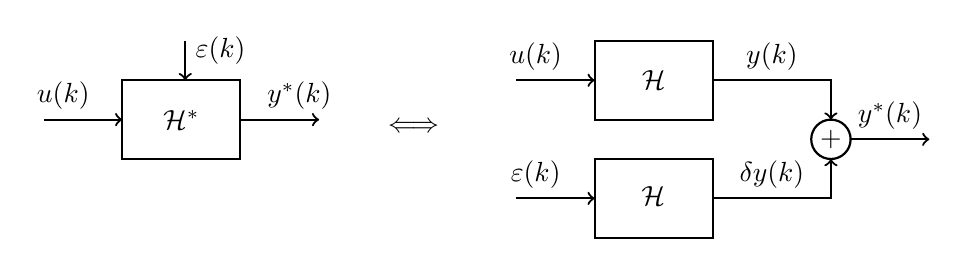
\begin{tikzpicture}[x=1cm,y=1cm]
				\draw (-9, 0.5) -- (-8,0.5) [->, thick] node[above,near start]{$\boldsymbol{u}(k)$};
				\draw (-7.2, 1.5) -- (-7.2,1.0) [->, thick] node[right,near start]{$\boldsymbol{\varepsilon}(k)$};
				\draw (-6.5, 0.5) -- (-5.5,0.5) [->, thick] node[above,near end]{$\boldsymbol{y}^*(k)$};
				\draw (-8,0.0) rectangle ++(1.5,1)[thick] node [midway]{$\mathcal{H}^*$}; 
				\draw (-2,0.5) rectangle ++(1.5,1)[thick] node [midway]{$\mathcal{H}$}; 
				\draw (-3, 1) -- (-2,1) [->, thick] node [above,near start]{$\boldsymbol{u}(k)$}; 
				\draw (-0.5, 1)  -- (1,1) -- (1,0.5) [->, thick] node[xshift=-0.75cm,yshift=0.8cm]{$\boldsymbol{y}(k)$}; 

				\draw (-2,-1) rectangle ++(1.5,1)[thick] node [midway]{$\mathcal{H}_{\abserr}$}; 
				\draw (-3, -0.5) -- (-2,-0.5) [->, thick] node[above,near start]{$\boldsymbol{\varepsilon}(k)$};
				\draw (-0.5, -0.5) -- (1,-0.5) -- (1,0) [->, thick] node [xshift=-0.75cm,yshift=-0.2cm]{$\boldsymbol{\delta y}(k)$}; 

				\draw (1,0.25) circle (0.25) [thick] node {$+$}; 
				\draw (1.25,0.25) -- (2.25,0.25)[->, thick] node [above,midway] {$\boldsymbol{y}^*(k)$};

				\node (arrow) at (-4.3,0.4) {$\iff$};
			  \end{tikzpicture}

			\caption{A signal view of the error propagation with respect to the ideal filter \label{fig:ltierror}}
			\end{figure}


		According to \ref{zmatrix}:

		\begin{equation} \label{zepsmatrix}
		\boldsymbol{Z_\varepsilon}=
					\begin{pmatrix}
						\boldsymbol{-J} & \boldsymbol{M} & \boldsymbol{M}_t \\
						\boldsymbol{K} & \boldsymbol{P} & \boldsymbol{M}_x \\
						\boldsymbol{L} & \boldsymbol{R} & \boldsymbol{M}_y 
					\end{pmatrix}
		\end{equation}

		with:
		\begin{eqnarray} \label{deltaerr}
			\boldsymbol{M}_t=(\boldsymbol{I}_{n_t} \hspace{5pt} \boldsymbol{0}_{n_t \times n_x} \hspace{5pt} \boldsymbol{0}_{n_t \times n_y}), \\
			\boldsymbol{M}_x=(\boldsymbol{0}_{n_x \times n_t} \hspace{5pt} \boldsymbol{I}_{n_x} \hspace{5pt} \boldsymbol{0}_{n_x \times n_y}), \\
			\boldsymbol{M}_y=(\boldsymbol{0}_{n_y \times n_t} \hspace{5pt} \boldsymbol{0}_{n_y \times n_x} \hspace{5pt} \boldsymbol{I}_{n_y}),
		\end{eqnarray}

		$\mathcal{H}_{\boldsymbol{\varepsilon}}$ is a filter with ($n_t+n_x+n_u$) inputs and $n_y$ outputs.
		\begin{proposition}
			The transfert function of filter $\mathcal{H_{\boldsymbol{\varepsilon}}}$, denoted $\boldsymbol{H}_\varepsilon$, is defined as follows:
			\begin{equation}
				\boldsymbol{H}_{\varepsilon}: \rightarrow \boldsymbol{C_Z}(z\boldsymbol{I}_n-\boldsymbol{A_Z})^{-1}\boldsymbol{M}_1 +\boldsymbol{M}_2 \hspace{5pt} \forall z \in \mathbb{C}
			\end{equation}
			with $\boldsymbol{A_Z}$ and $\boldsymbol{C_Z}$ the matrices defined by \ref{abcdtranspose} and
			\begin{equation}
				\boldsymbol{M_1}=(\boldsymbol{KJ}^{-1}   \hspace{10pt}\boldsymbol{I}_{n_x} \hspace{10pt} \boldsymbol{0}), \hspace{5pt}
				\boldsymbol{M_2}=(\boldsymbol{LJ}^{-1}  \hspace{10pt}\boldsymbol{0} \hspace{10pt}\boldsymbol{I}_{n_y}), 
			\end{equation}
		\end{proposition}
		The demonstration is well detailed in Lopez' PhD \cite{lopez}.

		\begin{corollary} \label{corimp}
			Considering a filter $\mathcal{H}$, $\boldsymbol{\varepsilon}(k)$ the vector of computation errors at time $k$ in the finite precision of $\mathcal{H}$,
			and $\mathcal{H}\boldsymbol{\varepsilon}$ the error filter associated to $\mathcal{H}$.
			The behaviour of error can be described from $\boldsymbol{\varepsilon}(k)$ and $\mathcal{H}\boldsymbol{\varepsilon}$.
			The error is considered as an interval vector, denoted by its center and radius $\langle \boldsymbol{\varepsilon}_m, \boldsymbol{\varepsilon}_r \rangle$ and 
			the interval vector of global error $\boldsymbol{\varepsilon}_y^*$, denoted $\langle {\boldsymbol{\varepsilon}_{y}^*}_m, {\boldsymbol{\varepsilon}_{y}^*}_r \rangle$.

			In practise, all inputs in our case are centered around zero, which is not the case in the control community, where this notation makes sense.
			So, $\boldsymbol{\varepsilon}_m=0$.
			The results are the following:

			\begin{eqnarray} \label{eqprec}
				{\boldsymbol{\varepsilon}_{y}^*}_m = 0 \\
				{\boldsymbol{\varepsilon}_{y}^*}_r = \langle\langle \mathcal{H}_{\boldsymbol{\varepsilon}} \rangle\rangle_{wcpg} \cdot \boldsymbol{\varepsilon}_r
			\end{eqnarray}
		\end{corollary}

		In the following ${\boldsymbol{\varepsilon}_{y}^*}_m$ won't be taken into account.

		Let's define:
			$$n'=n_t+n_x+n_y$$

		and:

			\begin{equation}
				\boldsymbol{v'}=
				\begin{pmatrix}
					\boldsymbol{t}(k+1) \\
					\boldsymbol{x}(k+1) \\
					\boldsymbol{y}(k)   \\
				\end{pmatrix}
			\end{equation}


		Then, following Lopez's computations, precisions are derived for every intermediate step:
		
		\begin{equation}
			|\boldsymbol{\varepsilon}_{y_i}^*| \leq \sum_{j=1}^{n'} | \langle\langle \mathcal{H}_{\boldsymbol{\varepsilon}} \rangle\rangle_{i,j}| \cdot \boldsymbol{2^{lsb_{v'_j}}}
		\end{equation}

		To formalize with a matricial formulation:
		\begin{equation}
			|\boldsymbol{\varepsilon}_y^*| \leq | \langle\langle \mathcal{H}_{\boldsymbol{\varepsilon}} \rangle\rangle| \cdot \boldsymbol{2^{lsb_{v'}}}
		\end{equation}


		To satisfy the condition \ref{condition}, $\xi$ is defined as the minimal error the user wants, which gives:
		\begin{equation}
			| \langle\langle \mathcal{H}_{\boldsymbol{\varepsilon}} \rangle\rangle| \cdot \boldsymbol{2^{lsb_{v'}}} < \xi
		\end{equation}

		Following Lopez's calculations, we end up with a set of constraints :
		\begin{equation} \label{constr}
			\boldsymbol{\mathfrak{A}} \cdot \boldsymbol{2}^{lsb_{v'}-msb_{v'}-1} < \boldsymbol{1}_{n_y}
			%\boldsymbol{D} \cdot \boldsymbol{2}^{lsb_{v'}-msb_{v'}-1} < \boldsymbol{1}_{n_y}
		\end{equation}

		Where :
		\begin{eqnarray}
			\boldsymbol{\mathfrak{A}}_{i,j}= | \langle\langle \mathcal{H}_{\boldsymbol{\varepsilon}} \rangle\rangle_{i,j} | \cdot \frac{\boldsymbol{2^{msb_{v'_j}+1}}}{\xi_i} %\\
			%\boldsymbol{D}_{i,j}= | \langle\langle \mathcal{H}_{\boldsymbol{\varepsilon}} \rangle\rangle_{i,j}| \cdot \frac{\boldsymbol{2^{msb_{v'_j}+1}}}{\xi_i}
		\end{eqnarray}

		And $v\in\{t,x,y\}$.

		 So, all $lsb_{v_i}$ from all $msb_{v_i}$ can  be deduced from \ref{constr}.
		As $msb_{v_i}$ can be deduced directly from $\langle\langle \mathcal{H} \rangle\rangle_{wcpg}$, choosing and computing each operator precision is possible through linear programming.

		%\TODO: check if this step is sufficient.

%		\subsubsection{A working solution to this problem}
%		A solution poposed in Lopez's PhD \cite{lopez}, is to consider the following reformulation of constraint \ref{constraint}.
%		We can give a stronger majoration, as follows:
%		\begin{equation}
%			\frac{\mathfrak{A}_{i1}}{\boldsymbol{2}^{msb_{v'_1}-lsb_{v'_1}+1}} + \frac{\mathfrak{A}_{i2}}{\boldsymbol{2}^{msb_{v'_2}-lsb_{v'_2}+1}} + \dots + \frac{\mathfrak{A}_{in'}}{\boldsymbol{2}^{msb_{v'_{n'}}-lsb_{v'_{n'}}+1}} < 1, \hspace{5pt} \forall 1 \leq i \leq n_y 
%		\end{equation}
		
